\subsection{Quality Requirements}

In this section we will describe the quality requirements for the game and
will briefly describe all requirements under each quality requirement.
Each requirement will be described with a quality attribute scenario that looks like this:

\begin{itemize}
	\item {\bf Source of stimulus:} Human, computer, or other actor that generates the stimulus
	\item {\bf Stimulus:} condition that needs to be considered when it arrives at a system
	\item {\bf Environment:} the stimulus occurs within certain conditions
	\item {\bf Artifact:} some artifact is stimulated 
	\item {\bf Response:} the activity undertaken after the arrival of the stimulus
	\item {\bf Response measure:} when the response occur, it should be measured in some fashion so that the requirement can be tested.
\end{itemize}

\begin{figure}[!hr]
	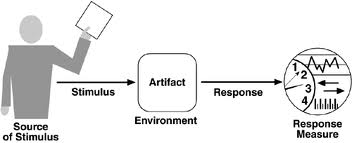
\includegraphics{pictures/qualityAttribute.jpg}
\end{figure}

{\bf What is a quality attribute?:}

{\bf Priority of quality attributes:} It is not possible to meet all quality requirements because some 
decisions will affect the other. This will result in a priority of the quality attributes that we need 
to meet and some others that are not that important. We have picked two main quality attributes: 
modifiability and performance.

\begin{itemize}
	\item {\bf Primary quality attribute: } Modifiability
	\item {\bf Secondary quality attributes: } Performance
\end{itemize}


\subsubsection{Modifiability}

Modifiability is about the cost of change. It brings up two concerns: What can change (the artifact)? 
When is the change made and who makes it (the environment)? 
Once a change has been specified, the new implementation must be designed, 
implemented, tested, and deployed. All of these actions take time and money, both of which can be measured.


{\bf M1: Add new elements} \\
In our game we have specified a small set of elements like powerplants, houses, powerlines, etc.
In order to have the oppertunity to add new buildings we have made a model for each element
with specific attributes. When e developer wants to add more elements, he/she can use the model
we have made and easily add the wanted parameters. 

\begin{tabular}{| l | l |}
	\hline
	Source of stimulus & \\ \hline
	Stimulus & \\ \hline
	Environment & \\ \hline
	Artifact & \\ \hline
	Response & \\ \hline
	Response Measure & \\ \hline
	
\end{tabular}

{\bf M2: Increase game difficulty}


\subsubsection{Performance}

{\bf P1: Rendering (Repaint)}

{\bf P2: Computational complexity}


\subsubsection{Other Quality attributes}
{\bf Usability: }

{\bf Testability:}

{\bf Compitability:}